% Options for packages loaded elsewhere
% Options for packages loaded elsewhere
\PassOptionsToPackage{unicode}{hyperref}
\PassOptionsToPackage{hyphens}{url}
%
\documentclass[
  12pt,
  letterpaper,
  DIV=11,
  numbers=noendperiod]{scrreprt}
\usepackage{xcolor}
\usepackage[margin=1in]{geometry}
\usepackage{amsmath,amssymb}
\setcounter{secnumdepth}{5}
\usepackage{iftex}
\ifPDFTeX
  \usepackage[T1]{fontenc}
  \usepackage[utf8]{inputenc}
  \usepackage{textcomp} % provide euro and other symbols
\else % if luatex or xetex
  \usepackage{unicode-math} % this also loads fontspec
  \defaultfontfeatures{Scale=MatchLowercase}
  \defaultfontfeatures[\rmfamily]{Ligatures=TeX,Scale=1}
\fi
\usepackage{lmodern}
\ifPDFTeX\else
  % xetex/luatex font selection
\fi
% Use upquote if available, for straight quotes in verbatim environments
\IfFileExists{upquote.sty}{\usepackage{upquote}}{}
\IfFileExists{microtype.sty}{% use microtype if available
  \usepackage[]{microtype}
  \UseMicrotypeSet[protrusion]{basicmath} % disable protrusion for tt fonts
}{}
\usepackage{setspace}
\makeatletter
\@ifundefined{KOMAClassName}{% if non-KOMA class
  \IfFileExists{parskip.sty}{%
    \usepackage{parskip}
  }{% else
    \setlength{\parindent}{0pt}
    \setlength{\parskip}{6pt plus 2pt minus 1pt}}
}{% if KOMA class
  \KOMAoptions{parskip=half}}
\makeatother
% Make \paragraph and \subparagraph free-standing
\makeatletter
\ifx\paragraph\undefined\else
  \let\oldparagraph\paragraph
  \renewcommand{\paragraph}{
    \@ifstar
      \xxxParagraphStar
      \xxxParagraphNoStar
  }
  \newcommand{\xxxParagraphStar}[1]{\oldparagraph*{#1}\mbox{}}
  \newcommand{\xxxParagraphNoStar}[1]{\oldparagraph{#1}\mbox{}}
\fi
\ifx\subparagraph\undefined\else
  \let\oldsubparagraph\subparagraph
  \renewcommand{\subparagraph}{
    \@ifstar
      \xxxSubParagraphStar
      \xxxSubParagraphNoStar
  }
  \newcommand{\xxxSubParagraphStar}[1]{\oldsubparagraph*{#1}\mbox{}}
  \newcommand{\xxxSubParagraphNoStar}[1]{\oldsubparagraph{#1}\mbox{}}
\fi
\makeatother


\usepackage{longtable,booktabs,array}
\newcounter{none} % for unnumbered tables
\usepackage{calc} % for calculating minipage widths
% Correct order of tables after \paragraph or \subparagraph
\usepackage{etoolbox}
\makeatletter
\patchcmd\longtable{\par}{\if@noskipsec\mbox{}\fi\par}{}{}
\makeatother
% Allow footnotes in longtable head/foot
\IfFileExists{footnotehyper.sty}{\usepackage{footnotehyper}}{\usepackage{footnote}}
\makesavenoteenv{longtable}
\usepackage{graphicx}
\makeatletter
\newsavebox\pandoc@box
\newcommand*\pandocbounded[1]{% scales image to fit in text height/width
  \sbox\pandoc@box{#1}%
  \Gscale@div\@tempa{\textheight}{\dimexpr\ht\pandoc@box+\dp\pandoc@box\relax}%
  \Gscale@div\@tempb{\linewidth}{\wd\pandoc@box}%
  \ifdim\@tempb\p@<\@tempa\p@\let\@tempa\@tempb\fi% select the smaller of both
  \ifdim\@tempa\p@<\p@\scalebox{\@tempa}{\usebox\pandoc@box}%
  \else\usebox{\pandoc@box}%
  \fi%
}
% Set default figure placement to htbp
\def\fps@figure{htbp}
\makeatother


% definitions for citeproc citations
\NewDocumentCommand\citeproctext{}{}
\NewDocumentCommand\citeproc{mm}{%
  \begingroup\def\citeproctext{#2}\cite{#1}\endgroup}
\makeatletter
 % allow citations to break across lines
 \let\@cite@ofmt\@firstofone
 % avoid brackets around text for \cite:
 \def\@biblabel#1{}
 \def\@cite#1#2{{#1\if@tempswa , #2\fi}}
\makeatother
\newlength{\cslhangindent}
\setlength{\cslhangindent}{1.5em}
\newlength{\csllabelwidth}
\setlength{\csllabelwidth}{3em}
\newenvironment{CSLReferences}[2] % #1 hanging-indent, #2 entry-spacing
 {\begin{list}{}{%
  \setlength{\itemindent}{0pt}
  \setlength{\leftmargin}{0pt}
  \setlength{\parsep}{0pt}
  % turn on hanging indent if param 1 is 1
  \ifodd #1
   \setlength{\leftmargin}{\cslhangindent}
   \setlength{\itemindent}{-1\cslhangindent}
  \fi
  % set entry spacing
  \setlength{\itemsep}{#2\baselineskip}}}
 {\end{list}}
\usepackage{calc}
\newcommand{\CSLBlock}[1]{\hfill\break\parbox[t]{\linewidth}{\strut\ignorespaces#1\strut}}
\newcommand{\CSLLeftMargin}[1]{\parbox[t]{\csllabelwidth}{\strut#1\strut}}
\newcommand{\CSLRightInline}[1]{\parbox[t]{\linewidth - \csllabelwidth}{\strut#1\strut}}
\newcommand{\CSLIndent}[1]{\hspace{\cslhangindent}#1}



\setlength{\emergencystretch}{3em} % prevent overfull lines

\providecommand{\tightlist}{%
  \setlength{\itemsep}{0pt}\setlength{\parskip}{0pt}}



 


\KOMAoption{captions}{tableheading}
\usepackage{chngcntr}
\counterwithout{equation}{chapter}
\counterwithout{footnote}{chapter}
\setkomafont{disposition}{\normalfont\bfseries}
\RedeclareSectionCommand[beforeskip=0pt,afterskip=1.2\baselineskip]{chapter}
\setlength{\emergencystretch}{3em}
\let\MRPListFigures\listoffigures
\let\MRPListTables\listoftables
\renewcommand{\listoffigures}{}
\renewcommand{\listoftables}{}
\makeatletter
\@ifpackageloaded{caption}{}{\usepackage{caption}}
\AtBeginDocument{%
\ifdefined\contentsname
  \renewcommand*\contentsname{Table of contents}
\else
  \newcommand\contentsname{Table of contents}
\fi
\ifdefined\listfigurename
  \renewcommand*\listfigurename{List of Figures}
\else
  \newcommand\listfigurename{List of Figures}
\fi
\ifdefined\listtablename
  \renewcommand*\listtablename{List of Tables}
\else
  \newcommand\listtablename{List of Tables}
\fi
\ifdefined\figurename
  \renewcommand*\figurename{Figure}
\else
  \newcommand\figurename{Figure}
\fi
\ifdefined\tablename
  \renewcommand*\tablename{Table}
\else
  \newcommand\tablename{Table}
\fi
}
\@ifpackageloaded{float}{}{\usepackage{float}}
\floatstyle{ruled}
\@ifundefined{c@chapter}{\newfloat{codelisting}{h}{lop}}{\newfloat{codelisting}{h}{lop}[chapter]}
\floatname{codelisting}{Listing}
\newcommand*\listoflistings{\listof{codelisting}{List of Listings}}
\makeatother
\makeatletter
\makeatother
\makeatletter
\@ifpackageloaded{caption}{}{\usepackage{caption}}
\@ifpackageloaded{subcaption}{}{\usepackage{subcaption}}
\makeatother
\usepackage{bookmark}
\IfFileExists{xurl.sty}{\usepackage{xurl}}{} % add URL line breaks if available
\urlstyle{same}
% fallback for those not using the hyperref driver hyperxmp:
\makeatletter
\@ifundefined{xmpquote}{\newcommand{\xmpquote}[1]{#1}}{}
\makeatother
\hypersetup{
  hidelinks,
  pdfcreator={LaTeX via pandoc}}


\author{}
\date{}
\begin{document}

\listoffigures
\listoftables

\setstretch{1}
\begin{titlepage}
\centering
\vspace*{1cm}
{\Large\bfseries Probabilistic Forecasting of Canadian Government Yields:\par}
\vspace{0.4cm}
{\Large\bfseries A Bayesian Stochastic-Volatility Extension of Dynamic Nelson--Siegel\par}
\vspace{1.6cm}
{\large Author: Ethan Yao\par}
\vspace{0.7cm}
October 2026\par
\vspace{0.7cm}
Supervisor: Greg Rice\par
\vfill
A project\par
In partial fulfilment of the requirement for\par
Master of Quantitative Finance\par
University of Waterloo\par

\end{titlepage}
\pagenumbering{roman}
\chapter*{Abstract}
\addcontentsline{toc}{chapter}{Abstract}

This study investigates whether stochastic factor volatility improves
probabilistic forecasts of Canadian government yields. Using weekly
yields at eight maturities, we compare Bayesian two-step Dynamic
Nelson--Siegel forecasts with constant and stochastic factor volatility
at 130 common expanding-window origins over 2016--2025. Stochastic
volatility DNS places a bounded prior on stationary log-volatility
variance; under the stated priors, this yields finite
posterior-predictive moments at finite horizons, so the predictive
covariance used in DSS exists.

Relative to constant volatility, stochastic volatility improves mean DSS
and Energy Score at both one and four-week horizons. At four weeks, its
Energy Score is 2.52\% lower, while pooled RMSE falls by only 0.162
basis points and the 95\% paired interval includes zero. The random walk
performs better than either Bayesian model on aggregate DSS, Energy
Score and RMSE. The results therefore indicate a modest
probabilistic-forecasting gain from stochastic volatility within the
matched DNS pair, not general predictive dominance. Because the
historical vintage and publication lag do not provide real-time
information sets, the findings are retrospective observation-time
comparisons.

\clearpage
\chapter*{Acknowledgements}
\addcontentsline{toc}{chapter}{Acknowledgements}

I am grateful to my supervisor, Greg Rice, for his guidance and feedback
throughout this project. I acknowledge the Bank of Canada as the source
of the Canadian zero-coupon yield-curve data.

\clearpage
\setcounter{tocdepth}{0}
\tableofcontents
\setcounter{tocdepth}{2}
\clearpage
\MRPListTables
\clearpage
\MRPListFigures
\clearpage
\pagenumbering{arabic}

\chapter{Introduction}\label{sec-introduction}

\section{Motivation and research
problem}\label{motivation-and-research-problem}

The term structure of interest rates describes the relationship between
government bond yields and their maturities, providing a fundamental
representation of interest-rate conditions across investment horizons.
Movements in the yield curve are rarely uniform: changes in monetary
policy expectations, inflation uncertainty, and macroeconomic conditions
may affect short, intermediate, and long-term yields differently. For
fixed-income portfolios, these movements translate into changes in bond
valuations and risk exposures that depend not only on the magnitude of
individual yield changes but also on their dependence across maturities.
Consequently, effective interest-rate risk measurement requires more
than forecasts of individual yields; it requires a coherent
representation of the joint distribution of future yield-curve
movements.

The Dynamic Nelson--Siegel (DNS) model represents the yield curve using
three factors: level, slope, and curvature. By reducing the
dimensionality of the term structure, DNS offers a tractable framework
for modeling yield dynamics and generating forecasts across maturities.
The dynamic forecasting approach developed by Diebold \& Li
(\citeproc{ref-diebold2006forecasting}{2006}) provides the foundation
for this study. However, conventional DNS specifications typically
assume constant factor-innovation variances, potentially limiting their
ability to represent changes in predictive uncertainty across different
interest-rate environments. In particular, periods of market instability
may be associated with substantially different volatility conditions
from those observed during more stable periods.

To address this limitation, this paper investigates a Bayesian
stochastic-volatility extension of the DNS framework, motivated by the
existing literature on stochastic-volatility yield-curve modeling,
including Hautsch \& Yang (\citeproc{ref-hautsch2012bayesian}{2012}).
The proposed approach retains the conventional two-step DNS factor
extraction procedure while introducing time-varying stochastic
volatility into the subsequent factor dynamics. Bayesian inference
provides a framework for estimating these volatility processes and
generating posterior-predictive distributions of future yield curves.
The objective is not to develop a new term-structure model, but to
examine whether a computationally tractable extension of established
methods can improve the representation of yield-curve uncertainty.

The central research question is whether incorporating Bayesian
stochastic volatility into DNS factor dynamics improves out-of-sample
probabilistic forecasts of Canadian government yields relative to
constant-volatility DNS specifications and conventional forecasting
benchmarks. The distinction between point forecasting and probabilistic
forecasting is central to this investigation. Models with similar
conditional mean forecasts may produce substantially different
predictive variances, covariance structures, and tail behavior.
Moreover, accurately reconstructing the observed yield curve does not
necessarily imply that a model can adequately characterize the
uncertainty surrounding its future evolution.

Accordingly, the empirical analysis emphasizes the quality of joint
predictive distributions rather than point-forecast accuracy alone.
Forecast performance is evaluated primarily through the multivariate
Gaussian quasi-likelihood, expressed as the Dawid--Sebastiani Score,
which assesses predictive means and covariance matrices. The Energy
Score provides a complementary assessment of the broader multivariate
predictive distribution, while prediction-interval coverage and root
mean squared error offer additional calibration and point-forecast
diagnostics. Using Canadian government yield data, the study examines
whether explicitly modeling stochastic factor volatility produces
measurable improvements in forecast uncertainty and whether such
improvements remain meaningful relative to simpler forecasting
alternatives.

\section{Contribution and scope}\label{contribution-and-scope}

This paper focuses on improving probabilistic yield-curve forecasting
within the DNS framework by introducing Bayesian stochastic volatility
into the factor dynamics. The study extends the conventional DNS
approach to examine whether modeling time-varying factor volatility
provides a better representation of forecast uncertainty. The main
comparison is between Bayesian DNS with constant factor volatility and
Bayesian DNS with stochastic factor volatility. Both models share the
same extracted factors, coefficient priors, forecast dates, and yield
reconstruction-error treatment, allowing the effect of stochastic
volatility to be evaluated within a consistent framework. The prior
specifications also preserve a common interpretation of long-run factor
innovation variance, while the bounded volatility prior ensures that the
required finite-horizon predictive moments exist under the stated model.

The empirical analysis uses Canadian government yield curves across 130
common out-of-sample forecast origins at one- and four-week horizons.
The results suggest that introducing stochastic volatility modestly
improves joint probabilistic forecasting within the Bayesian DNS
framework, although improvements in point-forecast accuracy remain
uncertain. Conventional forecasting methods, including the random walk,
PCA--VAR, and two-step Diebold--Li models, are included as external
benchmarks to place these findings in context, rather than as separate
methodological contributions. The random walk remains stronger on
aggregate forecasting metrics, highlighting the difficulty of improving
yield forecasts at short horizons.

The scope of this study is limited to evaluating probabilistic forecasts
within the DNS framework. It does not aim to establish that Bayesian DNS
models consistently outperform conventional forecasting approaches.
Further extensions, including joint Bayesian state-space estimation and
longer forecasting horizons, are left for future research.

\section{Organization}\label{organization}

Section~\ref{sec-literature} motivates the representation and scores.
Section~\ref{sec-data} defines the historical panel and information set.
Section~\ref{sec-methods} specifies the forecasting models and
finite-moment prior. Section~\ref{sec-design} describes the evaluation
and inference procedures. Section~\ref{sec-results} reports empirical
comparisons; Section~\ref{sec-discussion} interprets their scope and
limitations, followed by conclusions. Appendices provide derivations and
classical robustness results.

\chapter{Literature and conceptual framework}\label{sec-literature}

\section{DNS representation and conventional factor
forecasting}\label{dns-representation-and-conventional-factor-forecasting}

The DNS framework separates the cross-sectional representation of the
yield curve from the time-series dynamics of its factors. Diebold \& Li
(\citeproc{ref-diebold2006forecasting}{2006}) estimates level, slope and
curvature factors using fixed Nelson--Siegel loadings, then forecasts
those factors with autoregressions. Its reported gains are more
pronounced at a one-year horizon than at one month, underscoring that
performance depends on the forecasting horizon. The conventional
two-step DNS model provides the foundation for the present comparison.

The factors are interpreted through their maturity loadings: level loads
equally at every maturity, slope is strongest at short maturities and
approaches zero at long maturities, and curvature has a hump-shaped
loading. These labels describe the loading patterns; they do not
establish factor stationarity, cointegration or economic identification.
Factor extraction alone does not specify a predictive distribution;
assumptions about factor dynamics and innovations are also required.

PCA--VAR provides a secondary external comparison because its basis is
estimated from yield variation rather than imposed by the DNS loading
functions. Its factors need not share DNS's economic interpretation.
Differences between PCA--VAR and DNS can reflect the representation,
dynamics, covariance restrictions or parameter uncertainty, and
therefore do not isolate the contribution of stochastic volatility.

\section{Bayesian inference for DNS}\label{bayesian-inference-for-dns}

Bayesian DNS retains the two-step factor representation while assigning
probability distributions to factor-dynamic parameters.
Posterior-predictive forecasts integrate over parameter uncertainty,
unlike the plug-in forecasts of classical DNS. A constant-volatility
Bayesian specification is a useful control: it preserves the DNS
loadings and factor AR(1) mean structure while providing a direct
comparison for a stochastic-volatility extension.

The present models are two-step approximations. Extracted factors are
treated as observations in the second-stage Bayesian analysis, so
uncertainty in factor extraction and the fixed decay parameter is not
fully propagated. The results consequently concern Bayesian inference
conditional on the estimated factor representation, not a fully joint
latent-factor model.

\section{Stochastic factor
volatility}\label{stochastic-factor-volatility}

Stochastic-volatility DNS extends the constant-variance factor model by
allowing the log innovation variance to evolve over time. Hautsch \&
Yang (\citeproc{ref-hautsch2012bayesian}{2012}) studies Bayesian
stochastic volatility in monthly U.S. yield factors and reports
persistent factor volatility; Caldeira et al.
(\citeproc{ref-caldeira2010bayesian}{2010}) examines common and
factor-specific volatility structures for futures and Treasury yields.
These studies motivate allowing uncertainty to change across market
conditions, but they do not establish that the extension improves weekly
Canadian yield forecasts. Omori et al.
(\citeproc{ref-omori2007stochastic}{2007}) provides a mixture-based
approach to stochastic-volatility inference. The current model uses a
no-leverage restriction and evaluates the incremental forecasting value
of time-varying factor volatility within the same two-step DNS
framework.

The central comparison holds the factor extraction, factor AR mean
structure, coefficient priors, reconstruction-error treatment, forecast
dates and evaluation criteria fixed. It changes the factor
innovation-variance specification from constant to stochastic. This
controlled comparison is informative about that extension under the
stated assumptions, but it is not a causal effect separated from all
differences in the resulting volatility priors and predictive
distributions.

\section{Probabilistic forecast
evaluation}\label{probabilistic-forecast-evaluation}

Proper scoring rules motivate evaluating predictive distributions rather
than point forecasts alone (\citeproc{ref-gneiting2007strictly}{Gneiting
\& Raftery, 2007}). The Dawid--Sebastiani Score (DSS), introduced by
Dawid and Sebastiani (\citeproc{ref-dawid1999coherent}{Dawid \&
Sebastiani, 1999}), assesses the predictive mean and covariance, while
the Energy Score evaluates simulated multivariate yield vectors. DSS
cannot distinguish predictive distributions with identical first and
second moments; the Energy Score supplies complementary information but
is not a guarantee of correct tail dependence. The Variogram Score
emphasizes pairwise cross-maturity contrasts
(\citeproc{ref-scheuerer2015variogram}{Scheuerer \& Hamill, 2015}).
These scores complement marginal interval coverage and point-forecast
RMSE.

The score comparisons remain subject to finite-sample and
temporal-dependence uncertainty. Hansen et al.
(\citeproc{ref-hansen2011model}{2011}) introduces the Model Confidence
Set as one approach to forecast comparisons when predictive ability is
difficult to distinguish. Here it is reported only for the conventional
M0--M2 comparison; inference for the Bayesian pair uses paired
stationary-bootstrap intervals. Neither procedure establishes universal
model superiority.

\chapter{Data and information sets}\label{sec-data}

\section{Source and provenance}\label{source-and-provenance}

The primary source is the Bank of Canada's public zero-coupon
yield-curve series (\citeproc{ref-bocdata}{Bank of Canada, 2026}). Its
source page describes daily curves derived from Government of Canada
bonds and treasury bills, a quarterly maturity grid from 0.25 through 30
years, decimal yield units, missing observations marked \texttt{na}, and
a typical two-week update lag. These are estimated curves rather than a
panel of directly traded zero-coupon security prices at all maturities.
The Bank identifies Bolder et al.
(\citeproc{ref-bolder2004canadian}{2004}) as the methodology reference.

The supplied raw Canadian CSV is preserved separately from the processed
weekly panel. Its original retrieval transaction is not authenticated,
and the historical vintage may contain revisions. A separate
official-endpoint check found exact agreement for the eight maturities
on 21 complete December 2015 dates; this checks only that slice, not the
entire historical panel. Source evidence is retained under
\texttt{docs/sources/}; \texttt{src/prepare\_data.py} defines the
processor.

\section{Cleaning, units and weekly
sampling}\label{cleaning-units-and-weekly-sampling}

The selected maturity grid is \((0.25,0.5,1,2,5,7,10,30)\) years.
Headers are stripped of leading spaces; dates are parsed and checked for
uniqueness. A daily observation is eligible only if all eight selected
yields are present. The processor converts decimal yields to percentage
points by multiplying by 100 and selects the last eligible observation
in each ISO calendar week. This is neither averaging nor interpolation.

The research sample excludes the weekly observation dated 31 December
1999 and all dates in 2026. It contains 1,356 weekly observations: 835
through the end of 2015 and 521 in 2016--2025. Table~\ref{tbl-data}
summarizes this restricted sample. All scores use percentage-point
units; hence 0.01 percentage points equals one basis point. Comparisons
use identical units across models. Changing units shifts
determinant-based scores and rescales distance-based scores.

\begin{longtable}[]{@{}lllll@{}}
\caption{Weekly Canadian yields, 2000--2025, in percentage
points.}\label{tbl-data}\tabularnewline
\toprule\noalign{}
Maturity & Mean & SD & Min & Max \\
\midrule\noalign{}
\endfirsthead
\toprule\noalign{}
Maturity & Mean & SD & Min & Max \\
\midrule\noalign{}
\endhead
\bottomrule\noalign{}
\endlastfoot
0.250 & 2.109 & 1.612 & 0.049 & 5.756 \\
0.500 & 2.166 & 1.594 & 0.093 & 5.951 \\
1.000 & 2.261 & 1.568 & 0.123 & 6.166 \\
2.000 & 2.367 & 1.491 & 0.144 & 6.401 \\
5.000 & 2.733 & 1.451 & 0.294 & 6.484 \\
7.000 & 2.940 & 1.446 & 0.354 & 6.524 \\
10.000 & 3.179 & 1.404 & 0.482 & 6.556 \\
30.000 & 3.438 & 1.226 & 0.968 & 5.976 \\
\end{longtable}

\begin{figure}

\centering{

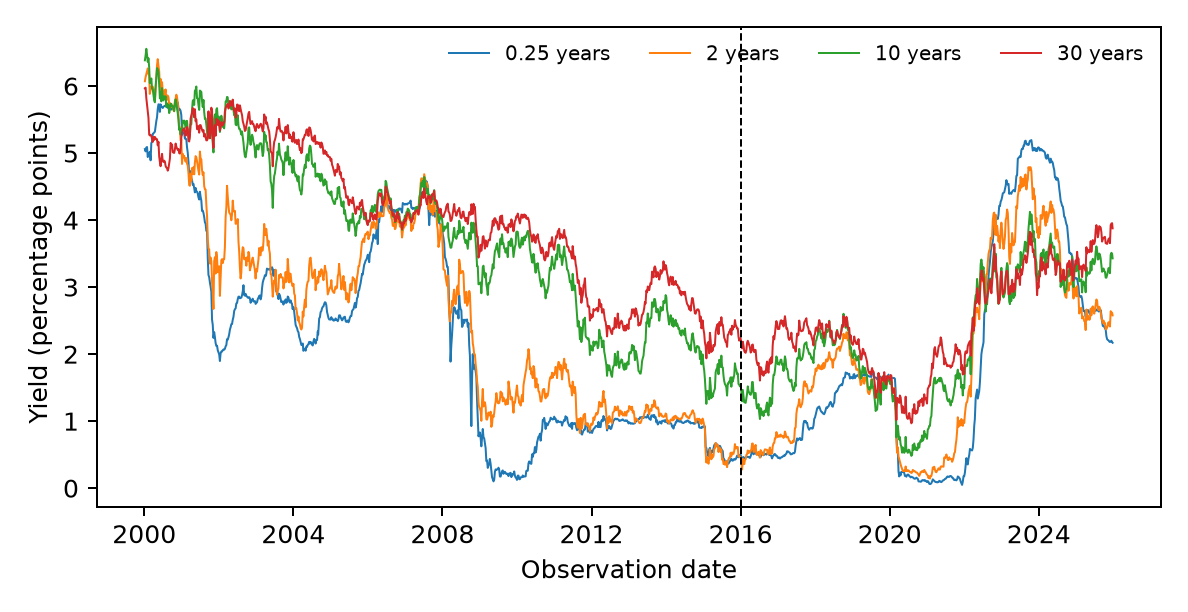
\includegraphics[width=0.95\linewidth,height=\textheight,keepaspectratio]{../figures/validated/yield_history.png}

}

\caption{\label{fig-history}Selected Canadian yield histories. The
vertical line marks the start of the evaluation period; observations are
not assumed publicly available contemporaneously.}

\end{figure}%

\section{Forecast dates and calendar
interpretation}\label{forecast-dates-and-calendar-interpretation}

Forecast horizons count weekly observations, not a fixed number of
trading days. Every fourth weekly observation in the out-of-sample
period is considered as an origin. An origin is retained only if both
its one- and four-observation-ahead targets lie in 2016--2025. This
gives 130 common origins, from 8 January 2016 to 28 November 2025. The
otherwise candidate observation near the end of December 2025 is
excluded because its four-week target is outside the sample.

Public holidays can change the weekday and elapsed calendar time between
observations without changing the weekly index. No interval between
successive observations exceeds ten calendar days. Accordingly, a
four-week forecast denotes four steps ahead in the weekly sample; its
target date follows from the observed calendar rather than a fixed
28-day interval.

\section{Observation-time versus publication-time
information}\label{observation-time-versus-publication-time-information}

The experiments fit models only to observations dated no later than the
origin. Lambda selection also uses only the initial training sample.
This prevents future-dated observation leakage within the supplied
historical panel. It does \textbf{not} establish a real-time forecasting
design.

The Bank's typical two-week publication lag means a curve dated \(t\)
would not normally be publicly available at \(t\). The later historical
vintage also leaves revision uncertainty. These are therefore
\textbf{retrospective observation-time forecasts}, not operational
forecasts under the public release-time information set. A real-time
backtest needs dated releases or a justified availability-lag rule; a
fixed lag alone cannot resolve revision uncertainty. No result is
interpreted as executable historical trading performance.

\chapter{Model specifications}\label{sec-methods}

\section{Nelson--Siegel observation
equation}\label{nelsonsiegel-observation-equation}

Let \(Y_t\) be the eight-dimensional yield vector and
\(f_t=(L_t,S_t,C_t)'\) the factors. For maturity \(\tau\) in years
define

\begin{equation}\protect\phantomsection\label{eq-loadings}{
s(\tau;\lambda)=\frac{1-e^{-\lambda\tau}}{\lambda\tau},
\qquad c(\tau;\lambda)=s(\tau;\lambda)-e^{-\lambda\tau}.
}\end{equation}

The row of the loading matrix at \(\tau\) is \((1,s,c)\). Level loads
equally at all maturities, slope declines toward zero at longer
maturities, and curvature has a hump-shaped loading. The observation
equation is

\begin{equation}\protect\phantomsection\label{eq-observation}{
Y_t=\Lambda(\lambda)f_t+\varepsilon_t,
\qquad \varepsilon_t\sim N(0,R_t).
}\end{equation}

The decay rate has units of inverse years; it is not a monthly
autoregressive parameter. A grid search over 160 values from 0.05
through 2.0 inverse years minimizes initial-window cross-sectional
squared error. The selected value, 0.516038 inverse years, is fixed
throughout the forecast exercise.

At each date the two-step factor estimator is

\begin{equation}\protect\phantomsection\label{eq-extraction}{
\widehat f_t=(\Lambda'\Lambda)^{-1}\Lambda'Y_t.
}\end{equation}

The factor estimator is obtained by least squares rather than by
explicitly forming the inverse. The maturity-specific diagonal of
\(R_t\) is the origin-specific mean squared reconstruction error,
floored at \(10^{-6}\) squared percentage points. This parsimonious
reconstruction-error model is shared across specifications; it does not
imply that actual residual errors are independent.

\section{Conventional two-step DNS}\label{conventional-two-step-dns}

M2 fits a separate Gaussian AR(1) mean equation to each extracted
factor:

\begin{equation}\protect\phantomsection\label{eq-ar}{
f_{j,t+1}=a_j+b_j f_{j,t}+\eta_{j,t+1},
\quad \eta_{j,t+1}\sim N(0,q_j).
}\end{equation}

For the classical benchmark the fitted intercept and slope are
unrestricted least-squares estimates. Conditional on fitted parameters,
factor forecast moments are

\begin{equation}\protect\phantomsection\label{eq-ar-moments}{
 m_{j,h}=b_j^h f_{j,t}+a_j\sum_{k=0}^{h-1}b_j^k,
\qquad v_{j,h}=q_j\sum_{k=0}^{h-1}b_j^{2k}.
}\end{equation}

The yield covariance is \(\Lambda\operatorname{diag}(v_h)\Lambda'+R_t\).
Parameter uncertainty is not added to this classical plug-in forecast.
Factor innovation independence is an explicit restriction; PCA--VAR
instead estimates a full covariance for its three factor innovations.

\section{Bayesian constant-volatility
DNS}\label{bayesian-constant-volatility-dns}

M3 is the primary control. It retains the factor AR(1) mean equation and
assumes a constant innovation variance \(\exp(m_j)\). Its coefficient
prior is

\begin{equation}\protect\phantomsection\label{eq-coefficient-prior}{
(a_j,b_j)'\sim N\!\left((0,0.7)',\operatorname{diag}(25,0.09)\right),\qquad |b_j|<1.
}\end{equation}

Here \(b_j\) controls factor persistence. The restriction \(|b_j|<1\) is
consistent with the stationary AR(1) specification. Before truncation,
its prior is centered at 0.7 with standard deviation 0.3, allowing a
broad range of moderately persistent dynamics. These choices are
inherited modeling assumptions, not parameters selected using test
scores.

The constant innovation variance has the prior

\begin{equation}\protect\phantomsection\label{eq-constant-variance-prior}{
m_j\sim N(\mu_{0j},25).
}\end{equation}

The parameter \(m_j\) is the log of the long-run expected factor
innovation variance. The center \(\mu_{0j}\) is calibrated from factor
residual variances in the initial 835-observation training sample and
held fixed across expanding windows. The same interpretation and
calibration are used in both Bayesian specifications. A standard
deviation of five on the log-variance scale is deliberately broad.
Because the initial observations calibrate the prior and also enter the
likelihood, this is an empirical-Bayes choice rather than independent
prior elicitation. Posterior-predictive simulation averages over
parameter draws, propagates future factor innovations and adds the
common reconstruction error, incorporating second-stage parameter
uncertainty omitted by classical M2.

\section{Bayesian DNS with stochastic factor
volatility}\label{bayesian-dns-with-stochastic-factor-volatility}

The main extension, M4, changes the factor innovation variance while
retaining the same factor extraction, maturity loadings, AR(1) mean
structure, coefficient priors, long-run expected-variance interpretation
and reconstruction-error treatment as M3:

\begin{equation}\protect\phantomsection\label{eq-sv-factor}{
f_{j,t}=a_j+b_j f_{j,t-1}+\eta_{j,t},
\qquad \eta_{j,t}\mid h_{j,t}\sim N(0,e^{h_{j,t}}),
}\end{equation}

\begin{equation}\protect\phantomsection\label{eq-sv-state}{
h_{j,t}=\omega_j+\phi_j(h_{j,t-1}-\omega_j)+u_{j,t},
\qquad u_{j,t}\sim N(0,\sigma_{u,j}^2).
}\end{equation}

The latent state \(h_{j,t}\) allows the factor innovation variance to
change over time. Its persistence parameter has the transformed prior

\begin{equation}\protect\phantomsection\label{eq-volatility-persistence-prior}{
\frac{\phi_j+1}{2}\sim\operatorname{Beta}(20,1.5),
\qquad E[\phi_j]=2\frac{20}{21.5}-1\approx0.86.
}\end{equation}

This transformation restricts \(\phi_j\) to \((-1,1)\), and the prior
favors persistent log volatility, a common feature of financial
volatility processes. The particular Beta hyperparameters remain
modeling choices.

To match the interpretation of \(m_j\) across M3 and M4, let \(v_j\) be
the stationary variance of log volatility and set

\begin{equation}\protect\phantomsection\label{eq-finite-reparam}{
\omega_j=m_j-v_j/2,\qquad \sigma_{u,j}^2=v_j(1-\phi_j^2),\qquad
h_{j,1}\sim N(\omega_j,v_j).
}\end{equation}

Then, under the stationary log-volatility process,
\(E[\exp(h_{j,t})\mid m_j,\phi_j,v_j]=\exp(m_j)\). The models share a
prior interpretation for long-run expected innovation variance, but not
their full predictive distributions: M4 additionally allows volatility
to vary over time.

For \(v_j\), the main specification uses a rate-one exponential prior
truncated to \((0,U)\):

\begin{equation}\protect\phantomsection\label{eq-finite-prior}{
p_U(v_j)=\frac{e^{-v_j}}{1-e^{-U}}\,1_{(0,U)}(v_j),
\qquad U=4.
}\end{equation}

The bound restricts stationary log-volatility variance to below four, or
its standard deviation to below two; it does not bound realized
volatility itself. The exponential density places more mass on smaller
\(v_j\), regularizing toward constant volatility. An untruncated
rate-one exponential would place \(e^{-4}\approx1.83\%\) probability
above four. Initial-window log-squared OLS residual variances are
approximately 4.87, 5.67 and 5.91, compared with about 4.935 for the
\(\log(\chi_1^2)\) noise variance. This is only a rough plausibility
check for latent variances of order one or smaller, not a fitted
stochastic-volatility variance estimate or evidence that \(U=4\) is
optimal. The bound is a modeling assumption; \(U=2\) and \(U=8\) are
evaluated at three representative origins only.

The bounded \(v_j\) prior and stated proper priors imply finite
posterior-predictive moments at each finite forecast horizon; the
appendix gives the argument. In particular, the predictive covariance
needed for DSS exists under these assumptions. This result does not
guarantee realistic uncertainty forecasts or good calibration, and
finite-horizon moments do not establish finite unconditional stationary
factor variance after mixing over coefficients arbitrarily close to a
unit root.

Posterior-predictive simulation propagates the factor and log-volatility
states at each future weekly step and adds the common reconstruction
error:

\begin{equation}\protect\phantomsection\label{eq-predictive}{
Y_{t+h}^{(s)}=\Lambda f_{t+h}^{(s)}+\varepsilon_{t+h}^{(s)},
\qquad \varepsilon_{t+h}^{(s)}\sim N(0,\widehat R_t).
}\end{equation}

The two-step method treats extracted factors as observations, so it does
not fully propagate first-stage factor-extraction or fixed-\(\lambda\)
uncertainty. Inference uses a Metropolis-corrected mixture sampler
targeting the exact likelihood, following Omori et al.
(\citeproc{ref-omori2007stochastic}{2007}).

\section{Conventional forecasting
benchmarks}\label{conventional-forecasting-benchmarks}

M0, the essential external benchmark, sets the future mean equal to the
current yield curve. At horizon \(h\), its covariance is the sample
covariance of overlapping historical \(h\)-step yield changes within the
expanding window. It is a zero-drift mean specification; covariance
eigenvalues follow the fixed training-only floor.

M1 provides secondary external context. It centers the expanding yield
panel, estimates its first three principal components, and fits a VAR(1)
with an intercept to their scores. For score dynamics
\(g_{t+1}=d+Ag_t+v_{t+1}\) with innovation covariance \(Q\), the
recursive forecast is

\begin{equation}\protect\phantomsection\label{eq-var-forecast}{
m_{k+1}=d+Am_k,\qquad V_{k+1}=AV_kA'+Q,
\quad m_0=g_t,\ V_0=0.
}\end{equation}

The yield mean adds the training center to the basis-projected score
mean; the covariance adds diagonal cross-sectional reconstruction error.
The PCA basis and VAR are refitted at every origin, and finite-horizon
forecasts do not impose a stationarity restriction on the estimated VAR.

\begin{longtable}[]{@{}
  >{\raggedright\arraybackslash}p{(\linewidth - 4\tabcolsep) * \real{0.3333}}
  >{\raggedright\arraybackslash}p{(\linewidth - 4\tabcolsep) * \real{0.3333}}
  >{\raggedright\arraybackslash}p{(\linewidth - 4\tabcolsep) * \real{0.3333}}@{}}
\caption{Forecasting specifications and their roles in the
comparison.}\label{tbl-ladder}\tabularnewline
\toprule\noalign{}
\begin{minipage}[b]{\linewidth}\raggedright
Model
\end{minipage} & \begin{minipage}[b]{\linewidth}\raggedright
Specification
\end{minipage} & \begin{minipage}[b]{\linewidth}\raggedright
Role in evaluation
\end{minipage} \\
\midrule\noalign{}
\endfirsthead
\toprule\noalign{}
\begin{minipage}[b]{\linewidth}\raggedright
Model
\end{minipage} & \begin{minipage}[b]{\linewidth}\raggedright
Specification
\end{minipage} & \begin{minipage}[b]{\linewidth}\raggedright
Role in evaluation
\end{minipage} \\
\midrule\noalign{}
\endhead
\bottomrule\noalign{}
\endlastfoot
M0 & Yield random walk; historical-change covariance & Essential
external benchmark \\
M1 & Three PCA factors with VAR(1) & Secondary external benchmark \\
M2 & Two-step DNS; independent Gaussian AR(1) factors & Conventional DNS
benchmark \\
M3 & Bayesian two-step DNS; constant factor volatility & Primary
control \\
M4 & Bayesian two-step DNS; finite-moment stochastic factor volatility &
Main extension \\
\end{longtable}

\chapter{Experimental design and evaluation}\label{sec-design}

\section{Expanding-window design}\label{expanding-window-design}

All models are evaluated on the same target curves and at the same two
horizons. Factor extraction, PCA centering, dynamics, residual
covariance and regularization use only observations dated no later than
each forecast origin. The initial 2000--2015 window selects \(\lambda\),
and the scoring period is 2016--2025. Common origins ensure comparisons
use the same interest-rate episodes.

The classical benchmarks yield 780 model--horizon--origin forecasts,
with predictive means and covariances computed analytically and 1,024
Gaussian scenarios used for ensemble scores. The Bayesian comparison
yields 520 forecasts: 130 origins, two horizons and two models. Each
Bayesian fit uses four chains, 3,000 warm-up iterations and 6,000
retained draws per chain, followed by 2,048 posterior-predictive
scenarios per model--horizon--origin.

Bayesian means and covariances use conditional analytic factor moments
averaged over posterior draws, including between-draw variation in
conditional means. Yield covariance adds the common reconstruction
covariance. Ensemble simulation propagates each future volatility and
factor step. This reduces moment-estimation noise without replacing the
non-Gaussian predictive scenarios used for Energy Score and intervals.

\section{Mean--covariance and Gaussian log
scores}\label{meancovariance-and-gaussian-log-scores}

For error \(e=Y_{t+h}-\widehat\mu_{t,h}\) the primary score is

\begin{equation}\protect\phantomsection\label{eq-dss}{
\operatorname{DSS}=\log|\widehat\Sigma|+e'\widehat\Sigma^{-1}e.
}\end{equation}

Smaller is better. Computation uses a Cholesky factor, triangular solves
and a log determinant rather than a direct inverse. Positive-definite
covariance is essential. If \(\Sigma\) is nearly singular, small errors
in maturity contrasts can generate large quadratic terms; a
low-dimensional fit alone does not guarantee a good DSS.

For an eight-dimensional Gaussian forecast the negative log density is

\begin{equation}\protect\phantomsection\label{eq-logscore}{
-\log p(Y)=\tfrac12\{8\log(2\pi)+\operatorname{DSS}\}.
}\end{equation}

For Gaussian classical forecasts this transformation is a negative log
density. For Bayesian mixtures it is only a Gaussian moment-based
quasi-log score, not an exact mixture log predictive density. This paper
therefore interprets DSS as a mean--covariance score and does not infer
a full mixture density ranking from it.

\section{Ensemble and marginal
evaluation}\label{ensemble-and-marginal-evaluation}

For predictive draws \(X^{(m)}\) and target \(y\), the Energy Score
estimate is

\begin{equation}\protect\phantomsection\label{eq-energy}{
\widehat{ES}=\frac1M\sum_{m=1}^M\|X^{(m)}-y\|
-\frac{1}{M(M-1)}\sum_{m<n}\|X^{(m)}-X^{(n)}\|.
}\end{equation}

The second term uses distinct draw pairs. This Monte Carlo estimator
targets the distributional Energy Score under independent predictive
simulation, rather than the finite-ensemble plug-in convention with an
\(M^2\) denominator. Both classical and Bayesian forecasts use the
distinct-pair convention, although their scenario counts differ and
therefore their Monte Carlo precision is not identical. Independent-seed
checks at representative origins assess Bayesian predictive stability;
the time-series bootstrap does not integrate MCMC or scenario-simulation
uncertainty.

Classical marginal central 90\% intervals use analytic Gaussian
quantiles. Bayesian intervals use the 5th and 95th percentiles of saved
mixture scenarios, not normal intervals reconstructed from the DSS
covariance. Coverage is pooled across maturities descriptively, while
inference resamples whole origins. Coverage is marginal, not
simultaneous eight-dimensional curve coverage. The classical Variogram
Score and PIT plots remain supplementary diagnostics; no new Bayesian
Variogram Score or formal PIT test is claimed.

Pooled RMSE is the square root of mean squared error across origins and
maturities, not the average of origin-level root mean squared errors.
MAE is the pooled mean absolute error. Percentages and percentage-point
quantities are kept distinct.

\section{Inference and computational
diagnostics}\label{inference-and-computational-diagnostics}

The primary comparison is the paired M4-minus-M3 score difference at
each common origin; lower DSS and Energy Score are better. We use a
stationary bootstrap (\citeproc{ref-politis1994stationary}{Politis \&
Romano, 1994}) with 9,999 replicates, an expected block length of eight
forecast origins and 95\% percentile intervals. Expected block lengths
of four and twelve assess sensitivity to the dependence assumption.
Geometrically distributed blocks preserve local temporal dependence;
block length is measured in forecast origins, not weeks.

Each resampled index vector selects both models, all maturities and the
same observed origins. RMSE is recomputed from resampled squared errors
before forming a difference. Thus an interval is not a bootstrap of
already-rooted origin errors, nor does it treat maturities as
independent dates. The stationary resampling scheme assumes the observed
loss dependence is informative about comparison uncertainty; structural
change in a decade-long rate sample is an important limitation.
Intervals are descriptive, unadjusted for multiple metrics or horizons,
and do not establish a population-wide model ranking.

Four-chain convergence is assessed using rank-normalized split
\(\widehat R\leq1.01\) and bulk and tail effective sample sizes of at
least 400 (\citeproc{ref-vehtari2021rank}{Vehtari et al., 2021}).
Synthetic recovery and independent-seed checks at initial, stress and
late windows assess sampler and predictive stability. At every origin,
predictive covariances are checked for positive definiteness and
forecast scores are reconstructed from the stored moments and scenarios.
These checks assess numerical reliability, not the economic adequacy of
the model.

For M0--M2, we report HAC summaries and a restricted Model Confidence
Set. That comparison has a different model universe and resampling
specification from the primary M3--M4 analysis.

\chapter{Empirical results}\label{sec-results}

\section{Forecast sample and
diagnostics}\label{forecast-sample-and-diagnostics}

The rolling evaluation contains 130 common origins and 520 Bayesian
model--horizon forecasts. The maximum rank-normalized \(\widehat R\) is
1.00760; the minimum bulk and tail effective sample sizes are 1,034.3
and 1,969.3. The conventional benchmarks use the same origins.

\section{Primary four-week
comparison}\label{primary-four-week-comparison}

\begin{longtable}[]{@{}llllll@{}}
\caption{Four-week forecasts at 130 common origins. M3 is Bayesian DNS
with constant factor volatility; M4 adds stochastic factor volatility.
Lower DSS, Energy Score and RMSE are better; marginal coverage targets
90\%. Width is mean central-90\% marginal interval width. One basis
point equals 0.01 percentage points.}\label{tbl-joint-h4}\tabularnewline
\toprule\noalign{}
Model & DSS & Energy & RMSE (bp) & Cover (\%) & Width (bp) \\
\midrule\noalign{}
\endfirsthead
\toprule\noalign{}
Model & DSS & Energy & RMSE (bp) & Cover (\%) & Width (bp) \\
\midrule\noalign{}
\endhead
\bottomrule\noalign{}
\endlastfoot
M0 & -36.006 & 0.351 & 21.318 & 87.115 & 63.372 \\
M1 & -24.394 & 0.370 & 21.966 & 86.635 & 61.934 \\
M2 & -21.453 & 0.418 & 23.563 & 93.173 & 91.777 \\
M3 & -21.450 & 0.418 & 23.577 & 93.077 & 92.143 \\
M4 & -21.840 & 0.407 & 23.415 & 94.327 & 92.719 \\
\end{longtable}

At four weeks, stochastic-volatility M4 improves mean DSS from −21.450
to −21.840 and Energy Score from 0.4178 to 0.4073 relative to
constant-volatility M3. The paired M4-minus-M3 differences are −0.3899
for DSS and −0.01053 for Energy Score; the latter is a 2.52\% reduction
from M3's mean score. The point-forecast change is smaller: pooled RMSE
falls from 23.577 to 23.415 basis points, a difference of −0.162 with a
95\% interval of {[}−0.464, 0.151{]}. Thus the main gain is in
distributional scores rather than clearly improved point accuracy.

The volatility estimates in Figure~\ref{fig-factor-volatility}
illustrate the time-varying uncertainty represented by M4. The figure
reports posterior estimates of terminal weekly factor innovation
standard deviations at each forecast origin, not direct observations of
volatility. The curvature-factor median rises sharply in 2022, reaches
60.6 basis points on 25 March 2022 and remains near that level in early
2023 before declining. Level and slope volatility also rise around 2022,
but less markedly.

\begin{figure}

\centering{

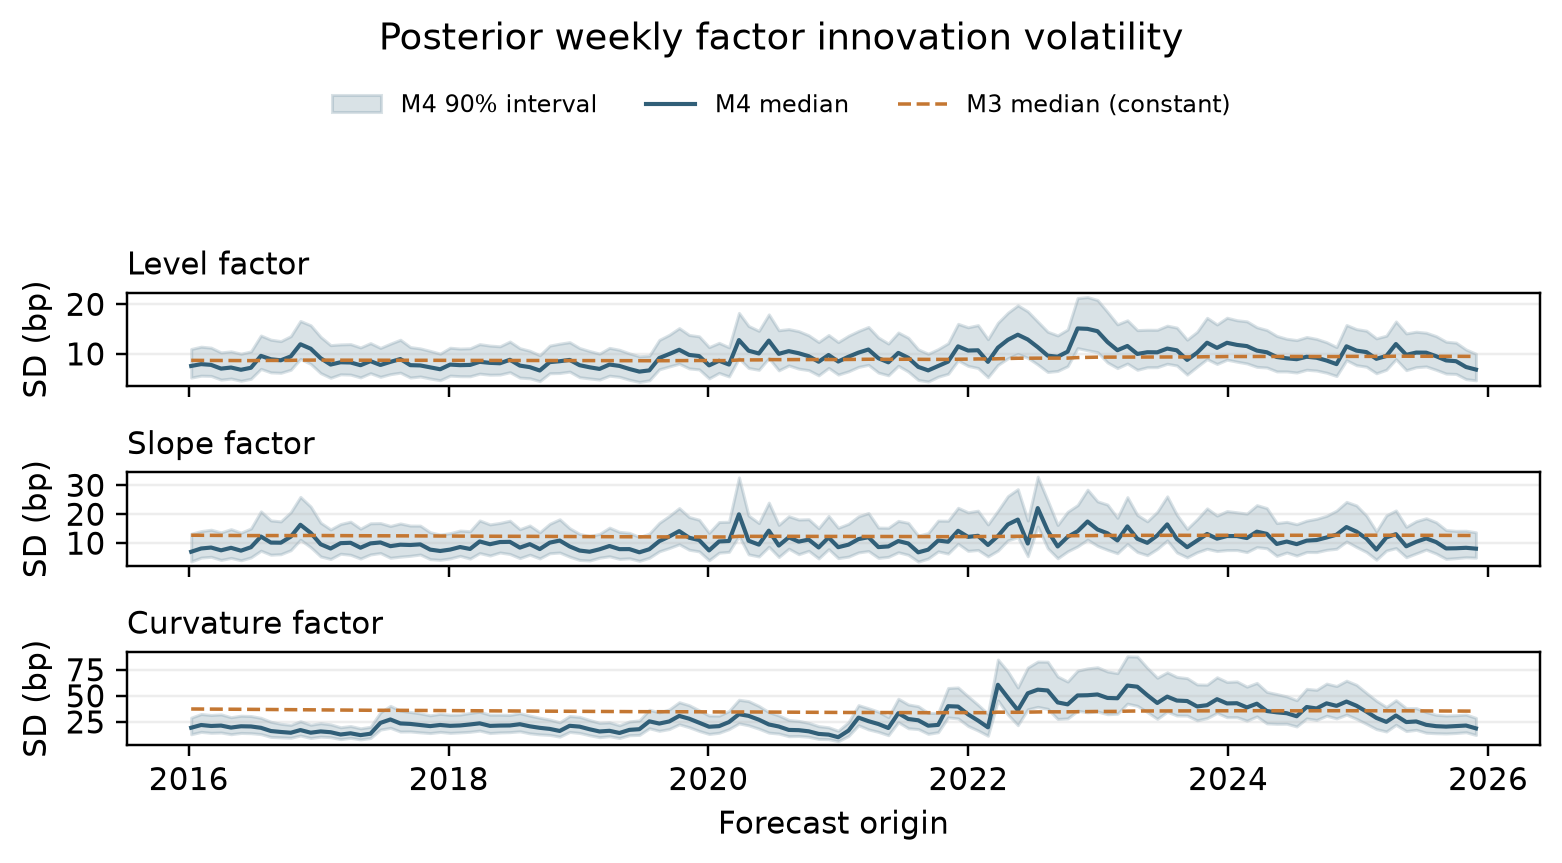
\includegraphics[width=0.95\linewidth,height=\textheight,keepaspectratio]{../figures/finite/presentation/estimated_factor_volatility.png}

}

\caption{\label{fig-factor-volatility}Posterior weekly factor innovation
standard deviations at 130 forecast origins, sampled every fourth week.
Shading gives the central 90\% posterior interval for M4; the dashed
line is the M3 posterior median, constant within each rolling fit.}

\end{figure}%

\section{One-week comparison}\label{one-week-comparison}

\begin{longtable}[]{@{}llllll@{}}
\caption{One-week forecasts at 130 common origins. M3 is Bayesian DNS
with constant factor volatility; M4 adds stochastic factor volatility.
Lower DSS, Energy Score and RMSE are better; marginal coverage targets
90\%. Width is mean central-90\% marginal interval width. One basis
point equals 0.01 percentage points.}\label{tbl-joint-h1}\tabularnewline
\toprule\noalign{}
Model & DSS & Energy & RMSE (bp) & Cover (\%) & Width (bp) \\
\midrule\noalign{}
\endfirsthead
\toprule\noalign{}
Model & DSS & Energy & RMSE (bp) & Cover (\%) & Width (bp) \\
\midrule\noalign{}
\endhead
\bottomrule\noalign{}
\endlastfoot
M0 & -41.223 & 0.163 & 9.972 & 90.481 & 30.811 \\
M1 & -29.095 & 0.205 & 11.722 & 90.481 & 34.218 \\
M2 & -25.370 & 0.255 & 13.858 & 94.423 & 52.482 \\
M3 & -25.357 & 0.256 & 13.876 & 94.423 & 52.580 \\
M4 & -25.648 & 0.252 & 13.883 & 94.712 & 52.709 \\
\end{longtable}

At one week, M4 reduces DSS by 0.291 and Energy Score by 0.00331, about
1.29\% of M3's mean Energy Score. The RMSE difference is +0.0064 basis
points and is not distinguishable from zero. The within-pair score
changes therefore have the same direction at both horizons, with a
larger Energy Score gain at four weeks.

\clearpage

\section{Paired uncertainty, calibration and maturity
patterns}\label{paired-uncertainty-calibration-and-maturity-patterns}

\begin{longtable}[]{@{}llll@{}}
\caption{Paired M4-minus-M3 stationary-bootstrap 95\% percentile
intervals: expected length eight origins, 9,999 replicates, seed 271026.
M3 has constant factor volatility; M4 has stochastic factor volatility.
Coverage differences are percentage points
(pp).}\label{tbl-finite-paired}\tabularnewline
\toprule\noalign{}
Horizon & Metric & M4 minus M3 & 95\% interval \\
\midrule\noalign{}
\endfirsthead
\toprule\noalign{}
Horizon & Metric & M4 minus M3 & 95\% interval \\
\midrule\noalign{}
\endhead
\bottomrule\noalign{}
\endlastfoot
1 & DSS & -0.291 & {[}-0.639, -0.011{]} \\
1 & Energy & -0.0033 & {[}-0.0053, -0.0013{]} \\
1 & RMSE (bp) & 0.006 & {[}-0.021, 0.038{]} \\
1 & Coverage (pp) & 0.29 & {[}-1.92, 2.69{]} \\
4 & DSS & -0.390 & {[}-0.762, -0.051{]} \\
4 & Energy & -0.0105 & {[}-0.0185, -0.0023{]} \\
4 & RMSE (bp) & -0.162 & {[}-0.464, 0.151{]} \\
4 & Coverage (pp) & 1.25 & {[}-1.06, 4.33{]} \\
\end{longtable}

The paired DSS and Energy Score intervals exclude zero in favor of M4 at
both horizons for the primary expected block length of eight origins.
RMSE and coverage-difference intervals contain zero. These are paired
time-series comparisons, not tests treating the 1,040 maturity--origin
cells as independent observations. At four weeks, the DSS interval is
{[}−0.762, −0.051{]} and the Energy Score interval is {[}−0.0185,
−0.0023{]}.

\begin{figure}

\centering{

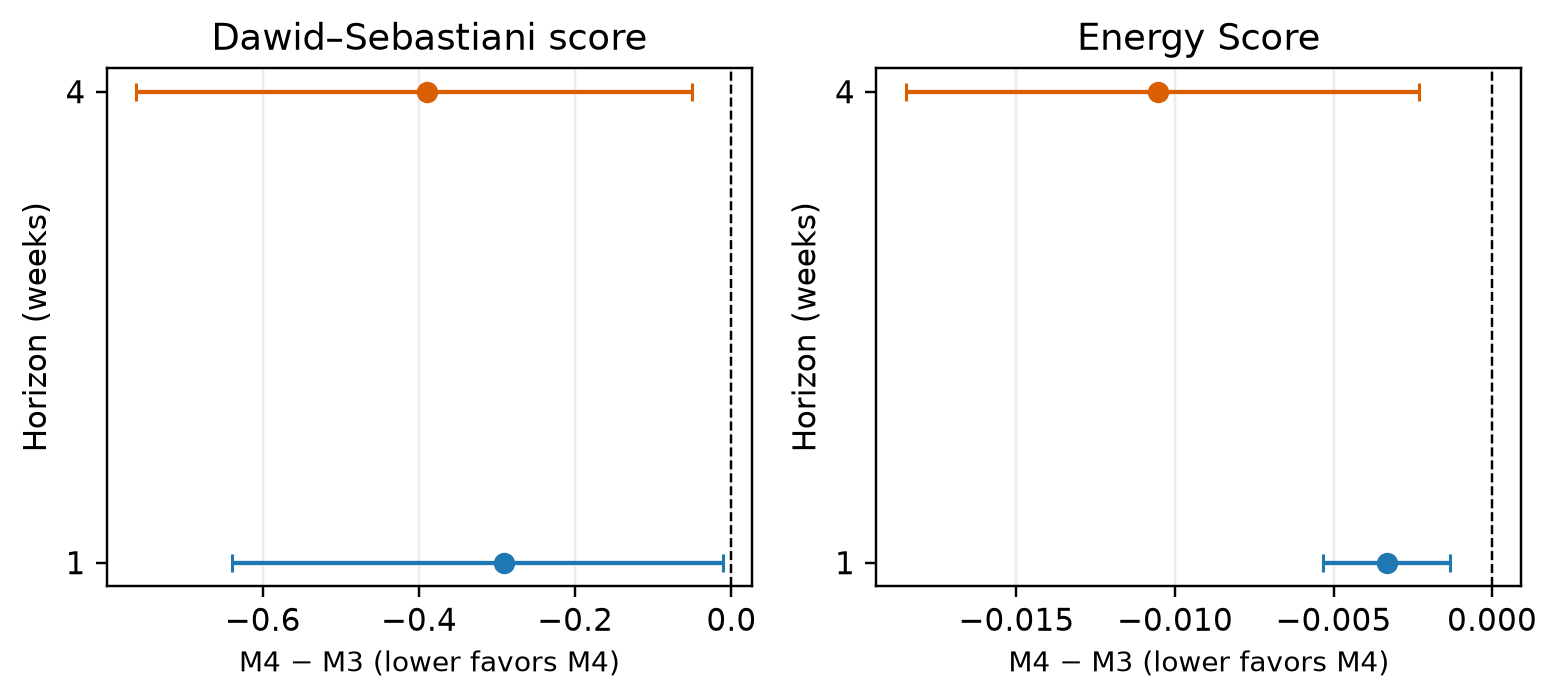
\includegraphics[width=0.95\linewidth,height=\textheight,keepaspectratio]{../figures/finite/presentation/paired_scores.png}

}

\caption{\label{fig-finite-paired}Paired M4-minus-M3 score differences
and 95\% stationary-bootstrap intervals, using expected block length
eight origins. Lower scores favor stochastic-volatility M4; the dashed
line is no difference. Each score has its own scale.}

\end{figure}%

\begin{longtable}[]{@{}
  >{\raggedright\arraybackslash}p{(\linewidth - 8\tabcolsep) * \real{0.2000}}
  >{\raggedright\arraybackslash}p{(\linewidth - 8\tabcolsep) * \real{0.2000}}
  >{\raggedright\arraybackslash}p{(\linewidth - 8\tabcolsep) * \real{0.2000}}
  >{\raggedright\arraybackslash}p{(\linewidth - 8\tabcolsep) * \real{0.2000}}
  >{\raggedright\arraybackslash}p{(\linewidth - 8\tabcolsep) * \real{0.2000}}@{}}
\caption{Dependence sensitivity: paired M4-minus-M3 score intervals
under expected stationary-bootstrap lengths 4, 8 and 12 origins, not
alternative prior bounds.}\label{tbl-finite-blocks}\tabularnewline
\toprule\noalign{}
\begin{minipage}[b]{\linewidth}\raggedright
Horizon
\end{minipage} & \begin{minipage}[b]{\linewidth}\raggedright
Loss
\end{minipage} & \begin{minipage}[b]{\linewidth}\raggedright
L=4
\end{minipage} & \begin{minipage}[b]{\linewidth}\raggedright
L=8
\end{minipage} & \begin{minipage}[b]{\linewidth}\raggedright
L=12
\end{minipage} \\
\midrule\noalign{}
\endfirsthead
\toprule\noalign{}
\begin{minipage}[b]{\linewidth}\raggedright
Horizon
\end{minipage} & \begin{minipage}[b]{\linewidth}\raggedright
Loss
\end{minipage} & \begin{minipage}[b]{\linewidth}\raggedright
L=4
\end{minipage} & \begin{minipage}[b]{\linewidth}\raggedright
L=8
\end{minipage} & \begin{minipage}[b]{\linewidth}\raggedright
L=12
\end{minipage} \\
\midrule\noalign{}
\endhead
\bottomrule\noalign{}
\endlastfoot
1 & DSS & {[}-0.6307, -0.0288{]} & {[}-0.6388, -0.0112{]} & {[}-0.6241,
-0.0097{]} \\
1 & Energy & {[}-0.0053, -0.0013{]} & {[}-0.0053, -0.0013{]} &
{[}-0.0052, -0.0013{]} \\
4 & DSS & {[}-0.7677, -0.0471{]} & {[}-0.7619, -0.0506{]} & {[}-0.7256,
-0.0586{]} \\
4 & Energy & {[}-0.0178, -0.0034{]} & {[}-0.0185, -0.0023{]} &
{[}-0.0183, -0.0025{]} \\
\end{longtable}

The score intervals remain below zero at expected block lengths four and
twelve. This supports the direction of the within-pair result under
these dependence assumptions, but does not remove uncertainty about
structural breaks, finite-sample bootstrap accuracy or multiple
comparisons. The one-week DSS upper endpoint is close to zero and should
not be overstated.

At four weeks, M3's pooled marginal 90\% coverage is 93.08\% and M4's is
94.33\%. M4 therefore moves farther above the nominal rate, not closer
to it. The coverage difference of 1.25 percentage points has a 95\%
interval containing zero. Mean interval width rises slightly, from
92.143 to 92.719 basis points. At one week, coverage is 94.42\% for M3
and 94.71\% for M4, with widths of 52.580 and 52.709 basis points. Both
models overcover in this pooled sense; improved proper scores do not
imply better marginal calibration or narrower forecasts.

\begin{figure}

\centering{

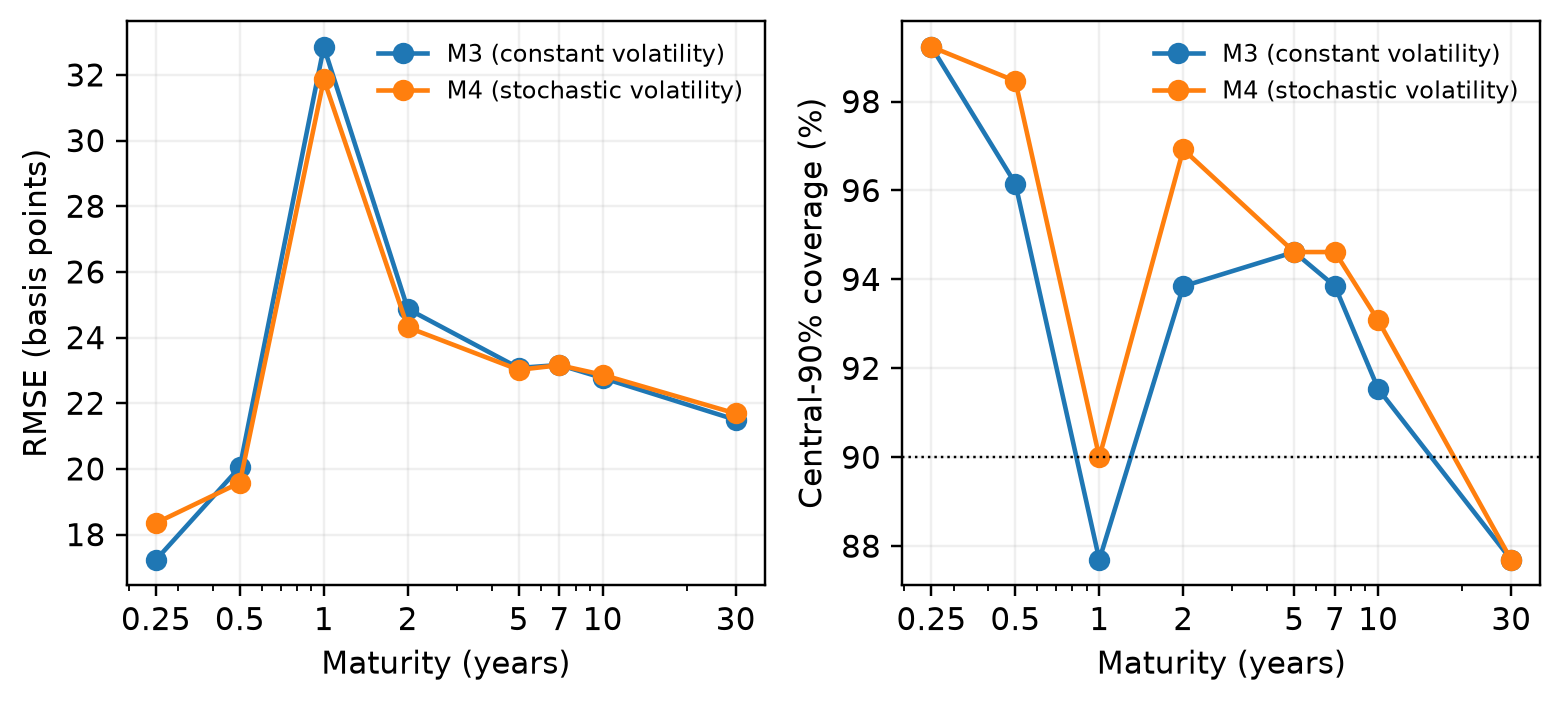
\includegraphics[width=0.95\linewidth,height=\textheight,keepaspectratio]{../figures/finite/presentation/maturity_h4.png}

}

\caption{\label{fig-finite-maturity}Four-week maturity-specific point
accuracy and marginal interval coverage for M3 and M4. The dotted
reference is 90\%; maturities are not independent replications.}

\end{figure}%

At four weeks, one-year coverage rises from 87.69\% under M3 to 90.00\%
under M4, while 30-year coverage is 87.69\% for both. RMSE changes
unevenly across maturities: M4 improves the one-year component but
worsens the three-month component. The pooled result is therefore not a
uniform maturity-by-maturity improvement.

\section{External benchmark
comparison}\label{external-benchmark-comparison}

The random walk M0 remains stronger than both Bayesian DNS models on
reported aggregate DSS, Energy Score and RMSE at both horizons. At four
weeks it has DSS −36.006, Energy Score 0.351 and RMSE 21.318 basis
points, compared with M4's 0.407 and 23.415 basis points for the latter
two measures. Its marginal coverage is lower (87.12\%) and its average
interval is narrower (63.37 versus 92.72 basis points), so lower scores
do not imply uniformly better calibration. PCA--VAR M1 also has lower
four-week DSS, Energy Score and RMSE than the Bayesian pair; M2 is the
conventional DNS reference. These external rankings are descriptive;
paired inference is conducted for M3 versus M4, not for all five
specifications.

\section{Prior-bound sensitivity}\label{prior-bound-sensitivity}

We evaluated \(U=2\) and \(U=8\) at the initial (8 January 2016), stress
(27 March 2020) and late (28 November 2025) origins. Constant-volatility
M3 is unchanged in these comparisons. This sensitivity analysis is
distinct from the block-length checks and covers three representative
origins, not all 130.

\begin{longtable}[]{@{}
  >{\raggedright\arraybackslash}p{(\linewidth - 10\tabcolsep) * \real{0.1667}}
  >{\raggedright\arraybackslash}p{(\linewidth - 10\tabcolsep) * \real{0.1667}}
  >{\raggedright\arraybackslash}p{(\linewidth - 10\tabcolsep) * \real{0.1667}}
  >{\raggedright\arraybackslash}p{(\linewidth - 10\tabcolsep) * \real{0.1667}}
  >{\raggedright\arraybackslash}p{(\linewidth - 10\tabcolsep) * \real{0.1667}}
  >{\raggedright\arraybackslash}p{(\linewidth - 10\tabcolsep) * \real{0.1667}}@{}}
\caption{Four-week representative prior-bound sensitivity. Differences
are M4 minus the unchanged cached M3 at the same origin. U=4 rows reuse
main forecasts; U=2/8 are the six accepted new cases. Single-origin
losses are descriptive, not full-sample
inference.}\label{tbl-finite-sensitivity}\tabularnewline
\toprule\noalign{}
\begin{minipage}[b]{\linewidth}\raggedright
Window
\end{minipage} & \begin{minipage}[b]{\linewidth}\raggedright
U
\end{minipage} & \begin{minipage}[b]{\linewidth}\raggedright
M4 DSS
\end{minipage} & \begin{minipage}[b]{\linewidth}\raggedright
M4 Energy
\end{minipage} & \begin{minipage}[b]{\linewidth}\raggedright
DSS diff. (M4 - M3)
\end{minipage} & \begin{minipage}[b]{\linewidth}\raggedright
Energy diff. (M4 - M3)
\end{minipage} \\
\midrule\noalign{}
\endfirsthead
\toprule\noalign{}
\begin{minipage}[b]{\linewidth}\raggedright
Window
\end{minipage} & \begin{minipage}[b]{\linewidth}\raggedright
U
\end{minipage} & \begin{minipage}[b]{\linewidth}\raggedright
M4 DSS
\end{minipage} & \begin{minipage}[b]{\linewidth}\raggedright
M4 Energy
\end{minipage} & \begin{minipage}[b]{\linewidth}\raggedright
DSS diff. (M4 - M3)
\end{minipage} & \begin{minipage}[b]{\linewidth}\raggedright
Energy diff. (M4 - M3)
\end{minipage} \\
\midrule\noalign{}
\endhead
\bottomrule\noalign{}
\endlastfoot
Initial & 2 & -24.582 & 0.3161 & -0.691 & -0.0227 \\
Initial & 4 & -24.581 & 0.3119 & -0.690 & -0.0269 \\
Initial & 8 & -24.585 & 0.3179 & -0.694 & -0.0209 \\
Stress & 2 & -21.063 & 0.3734 & 0.553 & 0.0402 \\
Stress & 4 & -21.055 & 0.3743 & 0.561 & 0.0412 \\
Stress & 8 & -21.053 & 0.3736 & 0.563 & 0.0404 \\
Late & 2 & -27.281 & 0.3310 & 0.651 & -0.0123 \\
Late & 4 & -27.276 & 0.3444 & 0.656 & 0.0010 \\
Late & 8 & -27.278 & 0.3360 & 0.655 & -0.0074 \\
\end{longtable}

At four weeks, changing the bound moves DSS by at most 0.00812 relative
to the main \(U=4\) forecasts. M4 has lower DSS initially but loses to
M3 at the stress and late origins. At one week, M3 has lower DSS at all
three representative dates under both alternative bounds. The positive
full-sample average result is therefore not a uniform improvement.

Energy Score rankings also change with the bound. At the late four-week
origin, the M4-minus-M3 difference is +0.0010 for \(U=4\), −0.0123 for
\(U=2\) and −0.0074 for \(U=8\). These representative cases support
local DSS stability, not uniform Energy Score improvement or full-period
prior robustness. No 130-origin comparison under alternative bounds was
performed, and the bound was not retuned.

\chapter{Discussion and limitations}\label{sec-discussion}

\section{What stochastic volatility
adds}\label{what-stochastic-volatility-adds}

The evidence answers a narrow but useful question. Conditional on the
shared two-step DNS representation, coefficient priors, long-run
expected-variance interpretation and reconstruction model, M4 improves
both covariance-sensitive DSS and ensemble-based Energy Score relative
to M3. Agreement between these criteria is more informative than DSS
alone because Energy Score uses simulated curve distances, while DSS
depends only on first and second moments. It does not establish that all
aspects of joint tail dependence are well represented.

At the primary four-week horizon, a 2.52\% Energy Score reduction is a
modest distributional improvement, not a large change in point accuracy.
Time-varying uncertainty can adapt forecasts while mean dynamics remain
nearly unchanged. This mechanism is consistent with the score and RMSE
pattern, but the experiment does not isolate a causal contribution from
particular episodes or factors.

\section{Why the random walk remains
competitive}\label{why-the-random-walk-remains-competitive}

At both horizons, the random walk has lower aggregate DSS, Energy Score
and RMSE than stochastic-volatility M4. Its RMSE is 9.972 basis points
at one week and 21.318 at four weeks, versus 13.883 and 23.415 for M4;
its four-week Energy Score is 0.351 versus 0.407. Its four-week marginal
90\% coverage is lower (87.12\% versus 94.33\%), however, and its mean
interval is narrower (63.37 versus 92.72 basis points). The lower scores
therefore do not imply uniformly better calibration.

Several design features could contribute, though the experiment does not
isolate their effects. The random walk forecasts each yield from its
latest value and estimates the eight-dimensional covariance directly
from historical changes, avoiding short-run mean estimation while
retaining observed cross-maturity co-movement. DNS instead uses a fixed
three-factor representation, factor AR dynamics, independent factor
innovations and diagonal reconstruction noise. These restrictions may
miss movements outside the factor span or in low-variance maturity
contrasts. Stochastic volatility adapts uncertainty but does not relax
these restrictions, so need not eliminate the associated forecast error.

Limited short-horizon predictability is one possible explanation, but it
is not directly tested. PCA--VAR also outperforms M4 on four-week DSS,
Energy Score and RMSE, so the external advantage is not specific to the
random-walk design. The paired bootstrap compares M4 only with M3;
external rankings are descriptive, not tests of superiority over the
random walk.

\section{Model and prior limitations}\label{model-and-prior-limitations}

Factors are extracted in a first stage and treated as observations
thereafter; uncertainty in extraction and in the fixed training-selected
decay rate is omitted. Independent factor innovations and diagonal
reconstruction noise restrict the predictive dependence structure.
Although forecasts are joint, these restrictions do not provide a fully
flexible eight-dimensional distribution. They can matter especially for
DSS in low-variance curve directions.

The finite-moment prior is an explicit change from an unrestricted
innovation-variance prior, not a purely numerical repair. Its bound is
required for the stated moment argument and must be part of the
scientific specification. Matching \(m\) aligns stationary
expected-variance priors, but does not match all higher moments. The
broad empirical-Bayes prior and its use of training data in both
hyperparameter calibration and the likelihood remain limitations.
Because the alternative-bound analysis covers only three selected
origins, it provides local rather than full-period sensitivity evidence.

Finite-horizon posterior-predictive moments do not establish finite
unconditional stationary factor variance under a coefficient-prior
mixture approaching \(|b|=1\). In the synthetic exercise, the 95\%
interval for the intercept did not contain its generating value. This
single replication is a computational diagnostic, not an assessment of
repeated-sampling coverage. Convergence diagnostics also establish
neither model truth nor the absence of all Monte Carlo error.

\section{Data, inference and practical
implications}\label{data-inference-and-practical-implications}

The observation-time experiment does not reconstruct real-time public
information. Publication delays and possible historical revisions
preclude an executable trading-performance interpretation. The existing
assumed-delay classical robustness exercise supports only the limited
historical-vintage conclusions reported in the appendix. A release-time
Bayesian comparison is not performed.

There are only 130 forecast origins across changing interest-rate
regimes. Stationary-bootstrap intervals are conditional descriptive
evidence under the declared dependence design, without multiplicity
correction or a model-confidence-set claim for the Bayesian pair. They
do not include uncertainty from choosing the representation or priors,
nor do they fully propagate numerical simulation uncertainty. Coverage
is marginal and descriptive; no formal joint-calibration or tail-risk
backtest is established.

For a researcher choosing between the two specified Bayesian DNS models,
M4 offers a small probabilistic-score improvement over M3. For an
applied forecaster choosing among the models studied here, the random
walk remains the strongest benchmark. Additional computation and
complexity should be justified by that external comparison, not merely
by a favorable within-family score.

\chapter{Conclusions}\label{sec-conclusions}

A comparison at 130 common Canadian yield-curve forecast origins finds
modest distributional value in finite-moment Bayesian stochastic
volatility. M4 improves DSS and Energy Score over matched
constant-volatility M3 at one and four weeks. At four weeks, the paired
DSS difference is −0.390 and Energy Score difference −0.0105; their
stationary-bootstrap intervals exclude zero, including under the
block-length sensitivity checks.

The economic and statistical qualifications matter. The four-week RMSE
gain is only 0.162 basis points and its interval includes zero. Both
Bayesian models overcover pooled marginal 90\% intervals, and M4 does
not beat the random walk on the reported aggregate scores. The main
finding is therefore a modest within-DNS probabilistic improvement, not
general model dominance or evidence of deployable trading gains.

Future work should prioritize genuinely release-time data, extraction
uncertainty and richer dependence or representation choices before
optional risk applications. Broader prior robustness and inference
across additional samples would assess how far the within-pair finding
generalizes. The contribution is a bounded finite-moment comparison
whose scope is deliberately limited to the matched Bayesian DNS pair;
the random-walk result remains the stronger external benchmark.

\appendix

\chapter{Analytical derivations and numerical
checks}\label{sec-appendix}

\section{Least-squares factor
extraction}\label{least-squares-factor-extraction}

For fixed \(\lambda\), minimize \(g(f)=(Y-\Lambda f)'(Y-\Lambda f)\).
Differentiation gives
\(\partial g/\partial f=-2\Lambda'Y+2\Lambda'\Lambda f\). Setting the
derivative to zero yields Equation~\ref{eq-extraction} when the three
columns have full rank. Least squares avoids explicitly computing an
inverse, which would be less stable if loadings were poorly conditioned.

As \(x=\lambda\tau\) approaches zero, \((1-e^{-x})/x\) approaches one.
The implementation uses \texttt{expm1} to avoid cancellation for small
positive \(x\). Curvature approaches zero at the short end. At long
maturities both nonlevel loadings approach zero. These limits establish
interpretation and basic sign checks; they do not identify factors
econometrically without further assumptions.

\section{AR and VAR forecast moments}\label{ar-and-var-forecast-moments}

Repeated substitution gives
\(f_{t+h}=b^hf_t+a\sum_{k=0}^{h-1}b^k+\sum_{k=0}^{h-1}b^k\eta_{t+h-k}\).
Taking expectations yields the mean in Equation~\ref{eq-ar-moments}.
Independent zero-mean innovations eliminate cross terms, giving
\(q\sum b^{2k}\) for its variance. The finite-sum form remains well
defined when a fitted slope is near one.

The matrix version replaces \(b^k\) with \(A^k\) and yields
Equation~\ref{eq-var-forecast}. If the origin state has filtered
covariance \(P_t\), an additional term \(A^hP_t(A^h)'\) appears,
accounting for uncertainty in the initial state.

\section{Yield predictive covariance}\label{yield-predictive-covariance}

For a fixed loading matrix and independent observation noise,
\(\operatorname{Var}(Y\mid\mathcal I_t)=\Lambda\operatorname{Var}(f\mid\mathcal I_t)\Lambda'+R_t\).
Reconstruction uncertainty is added once at the future observation, not
at every transition. In a Bayesian model, factor variance must include
both conditional innovation uncertainty and dispersion in conditional
means across posterior draws.

Estimating an eight-dimensional covariance from a small ensemble can add
noise in low-variance directions. Analytic addition of \(R_t\) to a
factor-level posterior covariance is a useful stability check, but
changing the estimator must be documented consistently. The classical
forecasts avoid this issue through exact fitted moments.

\section{Finite-moment prior and transformed
target}\label{finite-moment-prior-and-transformed-target}

For one factor, let \(n\) be the number of innovations and
\(e_t=h_t-\omega-\phi(h_{t-1}-\omega)\). With \(\omega=m-v/2\) and
\(q=v(1-\phi^2)\), the stationary path density has log form

\begin{equation}\protect\phantomsection\label{eq-finite-path}{
\begin{aligned}
\log p(h\mid m,\phi,v)={}&-\frac n2\log(2\pi)-\frac n2\log v
-\frac{n-1}{2}\log(1-\phi^2)\\
&-\frac{1}{2v}\left[(h_1-m+v/2)^2+\frac{\sum_{t=2}^n e_t^2}{1-\phi^2}\right].
\end{aligned}
}\end{equation}

The initial observation contribution cannot be omitted. The sampler
works in \(\theta=(m,u,s)\) with \(u=\operatorname{atanh}(\phi)\) and
\(s=\log v\). The independent-prior density gains Jacobian
\(\log(1-\phi^2)+s\). Equivalently, the determinant from these
coordinates to \((\omega,\phi,q)\) is \(v(1-\phi^2)^2\). The induced
physical-coordinate prior is not a product of the old independent priors
for \(\omega\) and \(q\).

At fixed \(m,\phi,h\), the \(v\) target contains
\(p_U(v)v^{-n/2}\exp[-A(v)/(2v)]\), where \(A(v)\) is the bracketed term
in Equation~\ref{eq-finite-path} and itself depends on \(v\). Thus it is
not the old inverse-gamma full conditional. Exact-target correction of
the reversible mixture proposal retains both the transformed prior and
this stationary density.

\section{Propriety and finite-horizon
moments}\label{propriety-and-finite-horizon-moments}

Conditional on the fixed empirical-Bayes hyperparameters, the factor
likelihood satisfies

\begin{equation}\protect\phantomsection\label{eq-likelihood-bound}{
L(x\mid a,b,h)\leq(2\pi)^{-n/2}\exp\!\left(-\frac12\sum_{t=1}^n h_t\right).
}\end{equation}

After integrating \(m\sim N(\mu_0,25)\), the log-volatility vector is
Gaussian conditional on \(v,\phi\), with mean \((\mu_0-v/2)\mathbf1\)
and covariance \(25\mathbf1\mathbf1'+vR_\phi\), where
\((R_\phi)_{ij}=\phi^{|i-j|}\). Every entry is bounded in absolute value
by \(25+U\). The logarithm of the expectation of the likelihood bound is
therefore bounded above by

\begin{equation}\protect\phantomsection\label{eq-normalizer-bound}{
-\frac{n\mu_0}{2}+\frac{nU}{4}+\frac{n^2(25+U)}8,
}\end{equation}

apart from the finite \((2\pi)^{-n/2}\) constant. Proper coefficient
priors and positivity on a set of positive prior probability give a
finite, strictly positive posterior normalizer.

Append a finite future log-volatility path. Multiplying the likelihood
bound by any finite exponential linear functional of this extended
Gaussian path still has a uniformly finite moment-generating function,
because \(v<U\). Hence future innovation variances have finite posterior
moments of all finite orders. At finite horizon \(H\), the factor mean
is bounded by \(|x_T|+H|a|\) since \(|b|<1\). The Gaussian intercept
prior has all polynomial moments. Gaussian innovation moments,
finite-sum inequalities and the exponential-moment bound then imply
finite-order posterior-predictive factor moments. Fixed linear loadings
and finite Gaussian reconstruction noise preserve this property for
yields. This finite-horizon statement does not integrate an
infinite-horizon factor variance proportional to \((1-b^2)^{-1}\).

\section{Conditional stochastic-volatility forecast
moments}\label{conditional-stochastic-volatility-forecast-moments}

At step \(k\), conditional on a posterior state,

\begin{equation}\protect\phantomsection\label{eq-sv-forecast-variance}{
E[e^{h_{T+k}}\mid\theta,h_T]
=\exp\!\left\{\omega+\phi^k(h_T-\omega)+\frac v2(1-\phi^{2k})\right\}.
}\end{equation}

The factor forecast mean is the AR expression in
Equation~\ref{eq-ar-moments}. Its conditional variance is the sum of
Equation~\ref{eq-sv-forecast-variance} weighted by \(b^{2(H-k)}\) for
\(k=1,\ldots,H\). Innovations at different future dates have zero cross
moments conditional on volatility, despite dependent volatility levels.
Averaging conditional variances and adding the posterior variance of
conditional means gives total factor predictive variance. Independent
factor posteriors yield a diagonal factor covariance; projection through
\(\Lambda\) and addition of \(R_t\) give the yield covariance used in
DSS.

Synthetic validation used a finite-moment generating specification and
independent chains. The true intercept, 0.04, lies just below the
retained interval {[}0.040314, 0.132335{]}. This interval miss is
reported rather than removed through tuning or repeated simulation.
Computational diagnostics do not imply that every realized credible
interval contains its generating value.

\section{Score reconstruction and data
integrity}\label{score-reconstruction-and-data-integrity}

The saved results comprise 780 classical and 520 Bayesian
model--horizon--origin records. Targets, posterior parameters, analytic
moments, scenario arrays and interval endpoints permit reconstruction
without refitting. Across the 130 origins, checks cover common keys,
covariance definiteness, interval reconstruction and DSS consistency;
independent Energy Score reconstruction is also performed at
representative origins. These checks establish consistency of the saved
calculations, not the truth of the modeling assumptions.

\section{Existing classical
robustness}\label{existing-classical-robustness}

The restricted M0--M2 90\% Model Confidence Set retains M0 at both
horizons for both reported losses. It does not compare the Bayesian pair
or all five specifications. Zero exceedances in a finite bootstrap
should not be read as a population probability of zero.

\begin{longtable}[]{@{}lll@{}}
\caption{Restricted 90\% Model Confidence Sets, range statistic,
stationary bootstrap with expected block length four origins, 1,999
replicates. Universe is M0--M2 only.}\label{tbl-mcs}\tabularnewline
\toprule\noalign{}
Horizon & Loss & Retained models \\
\midrule\noalign{}
\endfirsthead
\toprule\noalign{}
Horizon & Loss & Retained models \\
\midrule\noalign{}
\endhead
\bottomrule\noalign{}
\endlastfoot
1 & dss & M0 \\
1 & energy\_score & M0 \\
4 & dss & M0 \\
4 & energy\_score & M0 \\
\end{longtable}

A separate classical exercise excludes curves dated within 14 calendar
days of each origin and forecasts across the resulting bridge to the
original target. At four weeks, M0 remains the strongest classical
benchmark, with DSS −30.628 and pooled RMSE 0.275 percentage points.
This assumed-delay historical-vintage exercise is not a reconstruction
of exact historical publication dates or revisions, and it is not a
release-time M3--M4 comparison.

\begin{longtable}[]{@{}lllll@{}}
\caption{Four-week forecasts with an assumed 14-calendar-day
availability lag; 130 common origins. Historical vintages and exact
release dates are not recovered.}\label{tbl-availability}\tabularnewline
\toprule\noalign{}
Model & DSS & Energy & RMSE & Coverage \\
\midrule\noalign{}
\endfirsthead
\toprule\noalign{}
Model & DSS & Energy & RMSE & Coverage \\
\midrule\noalign{}
\endhead
\bottomrule\noalign{}
\endlastfoot
M0 & -30.628 & 0.459 & 0.275 & 0.869 \\
M1 & -22.669 & 0.466 & 0.277 & 0.866 \\
M2 & -20.182 & 0.511 & 0.293 & 0.930 \\
\end{longtable}

\chapter*{Bibliography}\label{bibliography}
\addcontentsline{toc}{chapter}{Bibliography}

\protect\phantomsection\label{refs}
\begin{CSLReferences}{1}{0}
\bibitem[\citeproctext]{ref-bocdata}
Bank of Canada. (2026). \emph{Yield curves for zero-coupon bonds}.
\url{https://www.bankofcanada.ca/rates/interest-rates/bond-yield-curves/}

\bibitem[\citeproctext]{ref-bolder2004canadian}
Bolder, D. J., Johnson, G., \& Metzler, A. (2004). \emph{An empirical
analysis of the canadian term structure of zero-coupon interest rates}
(Nos. 2004-48). Bank of Canada.
\url{https://publications.gc.ca/site/eng/9.559261/publication.html}

\bibitem[\citeproctext]{ref-caldeira2010bayesian}
Caldeira, J. F., Laurini, M. P., \& Portugal, M. S. (2010). Bayesian
inference applied to dynamic nelson-siegel model with stochastic
volatility. \emph{Brazilian Review of Econometrics}, \emph{30}(1),
123--161. \url{https://doi.org/10.12660/bre.v30n12010.3502}

\bibitem[\citeproctext]{ref-dawid1999coherent}
Dawid, A. P., \& Sebastiani, P. (1999). Coherent dispersion criteria for
optimal experimental design. \emph{The Annals of Statistics},
\emph{27}(1), 65--81. \url{https://doi.org/10.1214/aos/1018031101}

\bibitem[\citeproctext]{ref-diebold2006forecasting}
Diebold, F. X., \& Li, C. (2006). Forecasting the term structure of
government bond yields. \emph{Journal of Econometrics}, \emph{130}(2),
337--364. \url{https://doi.org/10.1016/j.jeconom.2005.03.005}

\bibitem[\citeproctext]{ref-gneiting2007strictly}
Gneiting, T., \& Raftery, A. E. (2007). Strictly proper scoring rules,
prediction, and estimation. \emph{Journal of the American Statistical
Association}, \emph{102}(477), 359--378.
\url{https://doi.org/10.1198/016214506000001437}

\bibitem[\citeproctext]{ref-hansen2011model}
Hansen, P. R., Lunde, A., \& Nason, J. M. (2011). The model confidence
set. \emph{Econometrica}, \emph{79}(2), 453--497.
\url{https://doi.org/10.3982/ecta5771}

\bibitem[\citeproctext]{ref-hautsch2012bayesian}
Hautsch, N., \& Yang, F. (2012). Bayesian inference in a stochastic
volatility nelson--siegel model. \emph{Computational Statistics \& Data
Analysis}, \emph{56}(11), 3774--3792.
\url{https://doi.org/10.1016/j.csda.2010.07.003}

\bibitem[\citeproctext]{ref-omori2007stochastic}
Omori, Y., Chib, S., Shephard, N., \& Nakajima, J. (2007). Stochastic
volatility with leverage: Fast and efficient likelihood inference.
\emph{Journal of Econometrics}, \emph{140}(2), 425--449.
\url{https://doi.org/10.1016/j.jeconom.2006.07.008}

\bibitem[\citeproctext]{ref-politis1994stationary}
Politis, D. N., \& Romano, J. P. (1994). The stationary bootstrap.
\emph{Journal of the American Statistical Association}, \emph{89}(428),
1303--1313. \url{https://doi.org/10.1080/01621459.1994.10476870}

\bibitem[\citeproctext]{ref-scheuerer2015variogram}
Scheuerer, M., \& Hamill, T. M. (2015). Variogram-based proper scoring
rules for probabilistic forecasts of multivariate quantities.
\emph{Monthly Weather Review}, \emph{143}(4), 1321--1334.
\url{https://doi.org/10.1175/mwr-d-14-00269.1}

\bibitem[\citeproctext]{ref-vehtari2021rank}
Vehtari, A., Gelman, A., Simpson, D., Carpenter, B., \& Bürkner, P.-C.
(2021). Rank-normalization, folding, and localization: An improved
{R-hat} for assessing convergence of {MCMC} (with discussion).
\emph{Bayesian Analysis}, \emph{16}(2), 667--718.
\url{https://doi.org/10.1214/20-BA1221}

\end{CSLReferences}




\end{document}
